\documentclass{article}
\usepackage[T1]{fontenc}
\usepackage{lmodern}
\usepackage{graphicx}
\usepackage{amsmath,amssymb}
\usepackage[a4paper,margin=2cm]{geometry}
\usepackage[absolute,overlay]{textpos}
\setlength{\TPHorizModule}{1mm}
\setlength{\TPVertModule}{1mm}
\usepackage[indonesian]{babel}
\usepackage{hyperref}
\setlength{\emergencystretch}{2em}
% unit: Halaman 49

\begin{document}

% === Halaman 49 (python/native) ===

49

PESAN RAHASIA :

KETEMUAN Di STASIUN KA 

MALAM JAM 13.00

0

00110011

10100010

11100010

01101111

111

00110010

10100011

11100011

01101111

Sumber: TA Yulie Anneria Sinaga 13504085

Pergeseran warna sebesar 1 dari 256 warna tidak dapat dilihat oleh manusia

% deskripsi: gambar native xref 235
\noindent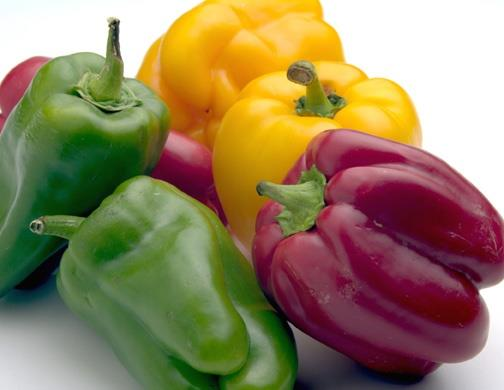
\includegraphics[width=0.85\textwidth]{../../images/python/page_049_img_01.jpeg}

\end{document}
